\documentclass[11pt, a4paper, oneside]{book}

% Um sprache umzustellen
% \usepackage[ngerman]{babel}
\usepackage[english]{babel}

% Restliche Settings einfügen
\usepackage{Setup/settings}

% Einstellungen für Metainformation in PDF-Datei
\hypersetup{pdftitle={ESC241 Pion and Muon lifetime},
            pdfauthor={Till Böhringer, Lucien Käser, Marc Urech, Richard Salnikov}}

% Was im Footer stehen soll, ifoot -> links, cfoot -> mitte
\ifoot{Pion and muon lifetimes}
\cfoot{ESC241}

% Allgemeine weite um alle Figures darauf zu beziehen
\newcommand\Plotwidth{0.8}
\newcommand\Bilderwidth{0.8}

% Setup wie siunix zahlen schreibt
\sisetup{group-separator = {'}, group-digits = integer}

% some stuff to make writing this report easiert
\newcommand{\electron}{$e^{-}$}
\newcommand{\pion}{$\pi^{-}$}
\newcommand{\muon}{$\mu^{-}$}

\lstset{language=python,
       basicstyle=\footnotesize\ttfamily,
  }

\begin{document}

% Bitte Titlepage noch bearbeiten falls nötig
\newgeometry{bottom=1cm, top=4cm} % die Abstände von oben und unten korrigieren
\begin{titlepage}
    \setlength{\headheight}{0cm}
	%\centering
	\includegraphics[width=0.45\textwidth]{\thelogofilename}\par\vspace{1cm}
    % \includesvg[width=0.45\textwidth]{\thelogofilename}\par\vspace{1cm}
	
	\centering
	
	{\bfseries\LARGE University of Zurich\par}
	\vspace{0.7cm}
	
	{\Huge\bfseries Pion and muon lifetimes\par}
	\vspace{0.7cm}

	{\LARGE Data analysis 2025 \par Group project IV \par }
	\vfill

    {\large Authors:\par\vspace{0.2cm}}
	{\Large\itshape Till Böhringer\\ \href{mailto:tillnils.boehringer@uzh.ch}{tillnils.boehringer@uzh.ch} \par
	\Large\itshape Lucien Käser\\ \href{mailto:luciendarian.kaeser@uzh.ch}{luciendarian.kaeser@uzh.ch} \par
	\Large\itshape Marc Urech\\ \href{mailto:marcandre.urech@uzh.ch}{marcandre.urech@uzh.ch} \par
	\Large\itshape Richard Salnikov\\ \href{mailto:richardivan.salnikov@uzh.ch}{richardivan.salnikov@uzh.ch} \par}
	\vfill

	
	{\large Lecturer:\par\vspace{0.2cm}}
	{\Large Patrick Owen}
	\vfill
	\vfill

% Bottom of the page
	{\large \today\par}
\end{titlepage}
\restoregeometry % das das restliche Dokument wieder die normale Geometrie hat
\frontmatter

\tableofcontents
\mainmatter

\chapter{Abstract}
% Short summary: goal, method, main results, ... 

\chapter{Introduction}
% what we want to do
In this project, a simplified simulation of an experiment will be performed to measure the lifetimes of pions (\pion) and muons (\muon) charges.

% problem description
\section{Motivation}
Negatively charged pions (\pion) are composite particles that consist of a down quark and an up antiquark. They are unstable and decay predominantly to a muon (\muon) and a muon-antineutrino ($\bar{v_{\mu}}$). The muon, a heavier partner of the electron, is also unstable and decays into an electron (\electron), a muon-neutrino ($v_{\mu}$) and an electron antineutrino ($\bar{v_{e}}$). Neglecting any experimental effects, the time distribution of the \electron produced in the decay chain is given by

\begin{equation}
    N(t) = \frac{N_0}{\tau_{\mu} - \tau_{\pi}}  \left[ \exp{-\frac{t}{\tau_{\mu}}} - \exp{-\frac{t}{\tau_{\pi}}} \right]
    \label{eq:decay_chain_equation}
\end{equation}



Where $\tau_{\mu}$ and $\tau_{\pi}$ are the mean lifetimes of the \muon and \pion respectively. A measurement of this time distribution allows extracting times for $\tau_{\mu}$ and $\tau_{\pi}$.

\section{Setup}

The basic elements of the corresponding real experiment are shown in Figure \ref{fig:experimental_setup} negatively charged pion (\pion) is stopped in the third scintillator. The electron emitted (\electron) is then detected in the fifth scintillator. The time difference between the moment the \pion is stopped in the third scintillator and the \electron is detected in the fifth scintillator is recorded. A spectrum of time differences for many such events will allow for an estimation of the half life times of the \pion ($\tau_{\pi}$) and the \muon ($\tau_{\mu}$).

\begin{figure}[h]
\begin{center}
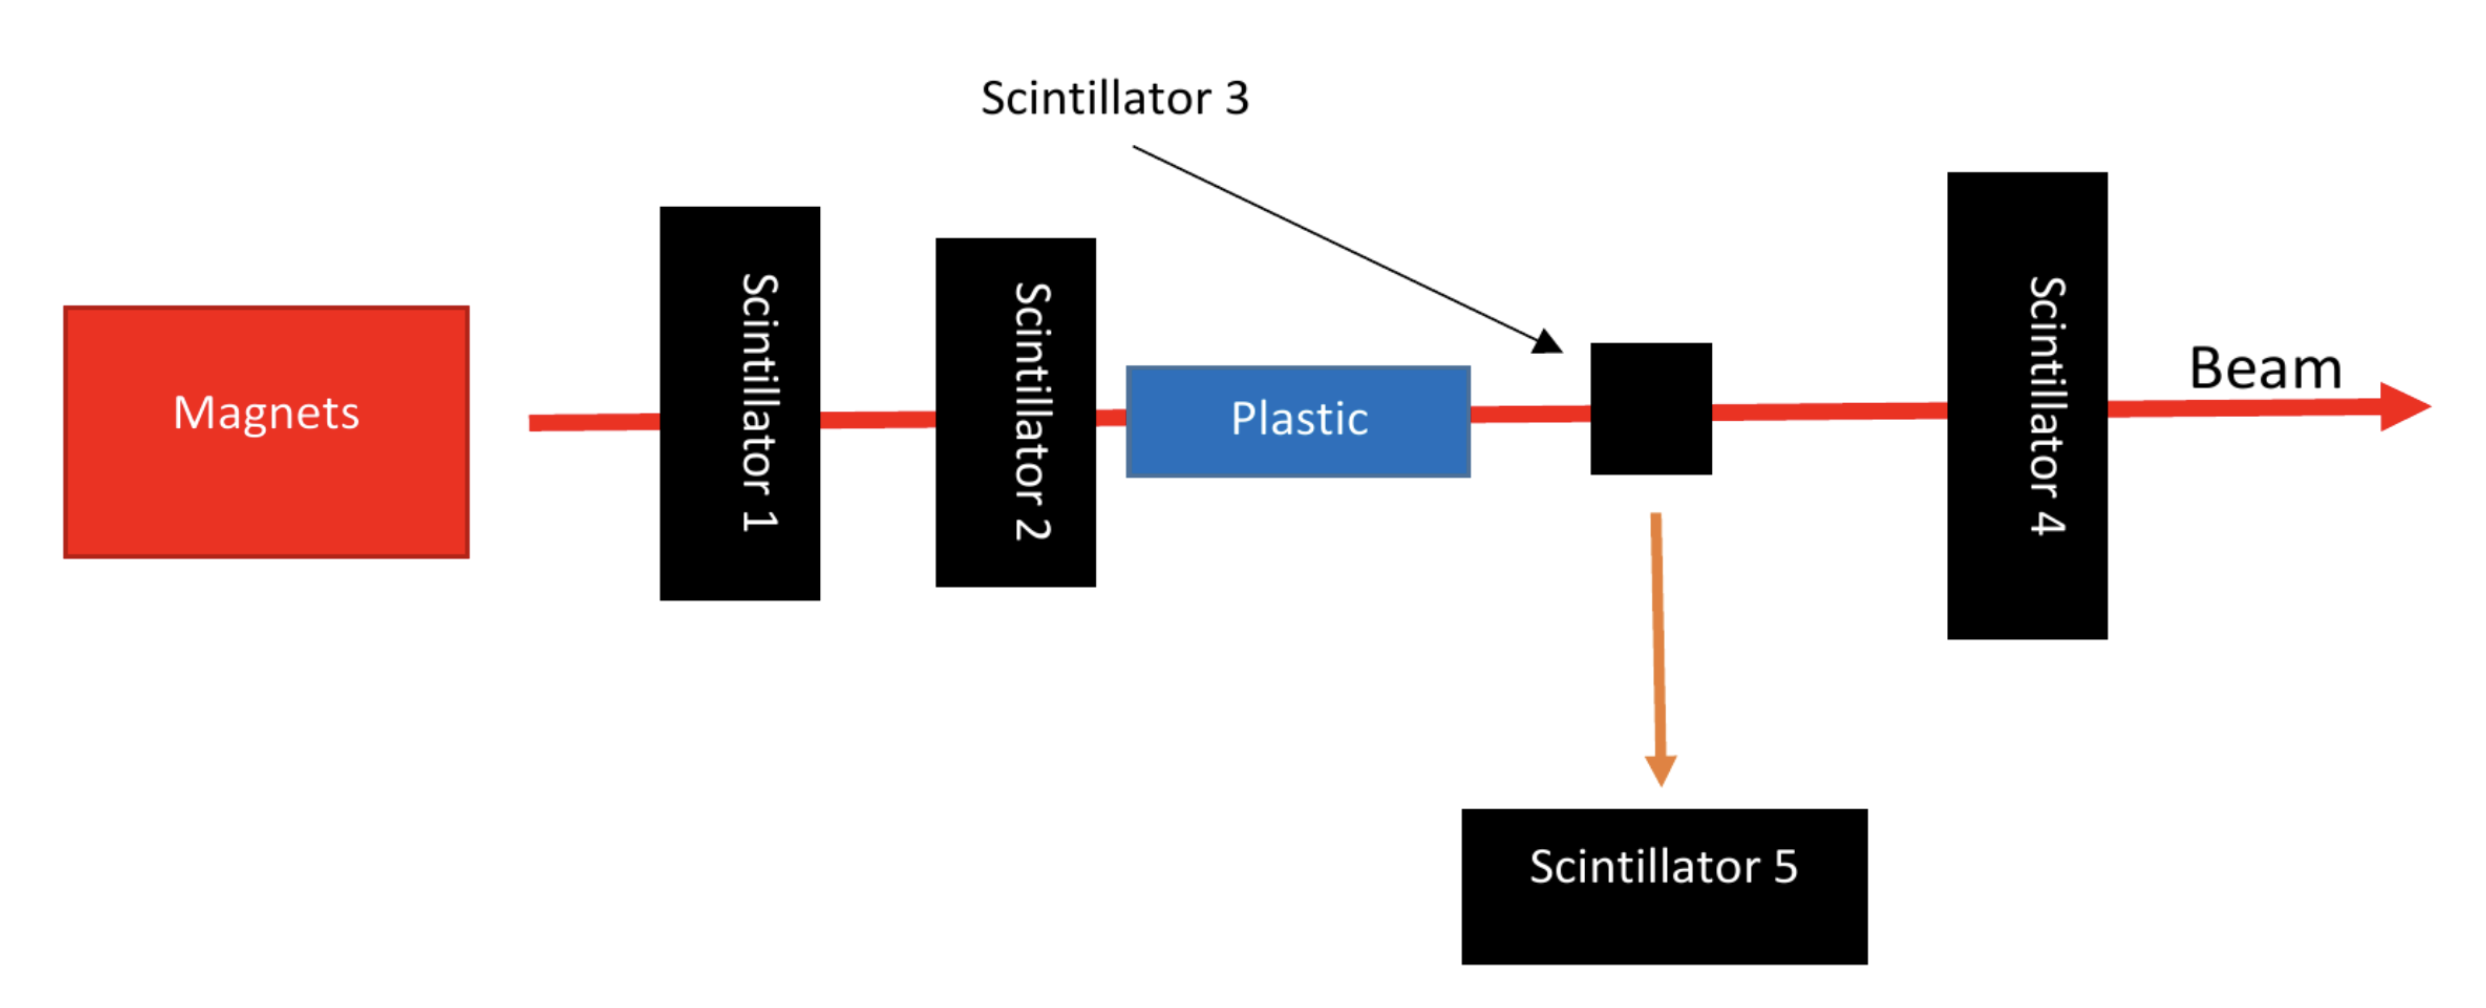
\includegraphics[width=0.7\textwidth]{images/experimental_setup.png}
\end{center}
\caption{Simplified sketch of the setup of the experiment (from the project documentation). A beam containing \pion passes through scintillators 1 and 2 and a piece of plastic to slow them down, such that they stop in scintillator 3. Scintillator 4 is a counter to reject events in which the beam particle was not stopped in scintillator 3. Electron \electron created in the decay chain are detected in scintillator 5. The signal from scintillator 3 starts a clock, the signal from scintillator 5 stops it.}
\label{fig:experimental_setup}
\end{figure}

% goal of the simulation
% short theoretical background

\FloatBarrier
\chapter{Methods}

In this chapter we go over the simulations we have done, at first a simple simulation and second a more realistic example.

\section{Simple simulation} \label{sec:simple_simulation}
% d\tau_{\pi}ription of the simulation model
% assumptions made
% algorithms or numerical methods used
% software / tools used

For the simple simulation, we simulated \num{10000} decays according to equation \ref{eq:decay_chain_equation} and known values from the Particle Data Group. \cite{ParticleDataGroup:2024cfk}

\pion Mean lifetime: \qty{2.6033(0.0005)e-8}{\s} \\
\muon Mean lifetime: \qty{2.1969811(0.0000022)e-6}{\s}

For the random sampling we generate random point from a constant distribution with width from \qty{0}{\s} to \qty{2e-5}{\s} and a height from 0 to the maximum counts of the distribution we want to sample from. We check if this point is in the desired distribution, if not, we generate a new random point, if it is in there, we return it. This we do until we have reached the desired amount of points in the distribution.

After we got all points generated, we draw a histogram, figure \ref{fig:histogram}.

\begin{figure}[h]
    \centering
    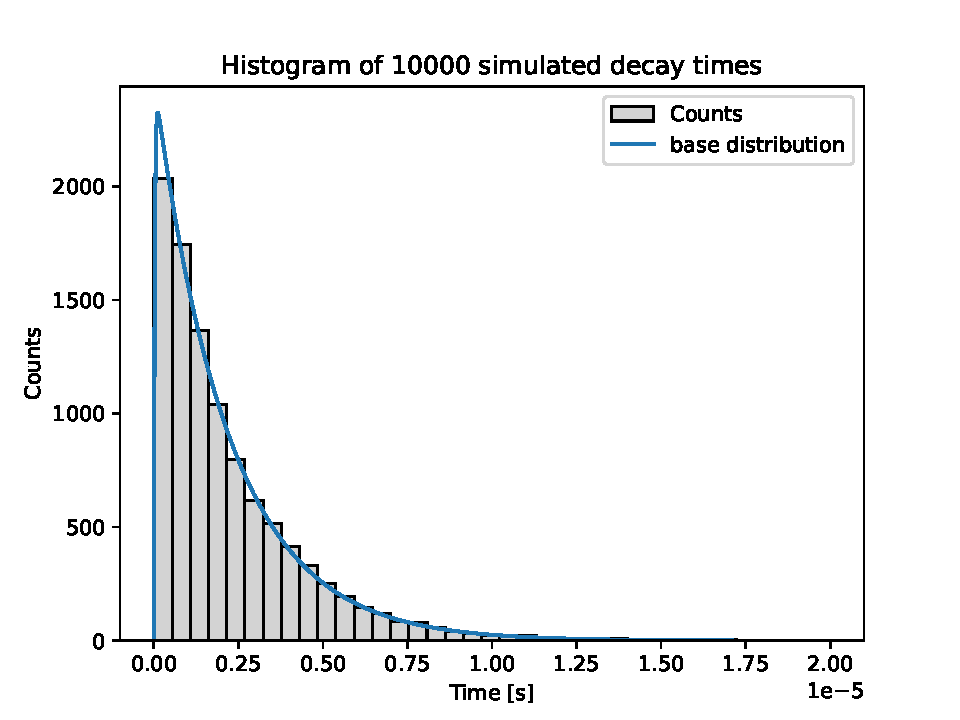
\includegraphics[width=\Plotwidth\textwidth]{images/simulated_decay_histogram.pdf}
    \caption{The histogram generated from random sampling the given distribution}
    \label{fig:histogram}
\end{figure}

Next we fitted back on the generated histogram the distribution, getting values for the lifetimes and corresponding uncertainties. The fitting was supposed to be done via a maximum likelihood fit, but as can be seen in figure \ref{fig:comparison_estimators}, the least squares method gives better results than the maximum likelihood fit. In figure \ref{fig:comparison_estimators} the maximum likelihood fit is implemented with the SciPy \lstinline{minimize} function, the least squares fit is done with the SciPy \lstinline{curve_fit} function and the full is a stack of fitters from \lstinline{dual_annealing} over a local \lstinline{minimize} to a custom Markov-chain minimizer.

\begin{figure}[h]
    \centering
    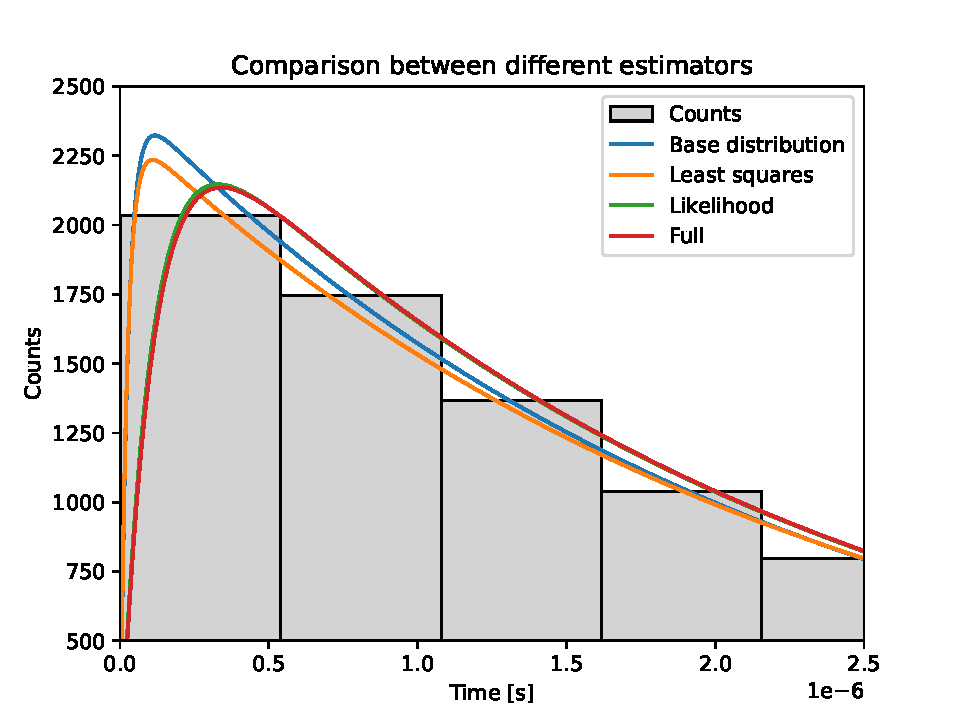
\includegraphics[width=\Plotwidth\textwidth]{images/comparison_estimators.pdf}
    \caption{Comparison between different estimators and the base distribution, overlaid on the histogram.}
    \label{fig:comparison_estimators}
\end{figure}

As can be seen in figure \ref{fig:comparison_estimators} the best representation of the base distribution gives the least squares fit, which we will use for the further exercises.

\section{A bit more realistic}

In section \ref{sec:simple_simulation}, the distribution of points were directly generated from the distribution \ref{eq:decay_chain_equation}. This isn't realistic, since the measurements itself aren't precise and have some noise to them. To implement this into the simulation, all simulated decay times got "smeared" by a random value drawn out of a normal distribution. The 

\chapter{Results}
% present key results (plots, tables, values)
% explain findings objectively, without interpretation

\chapter{Discussion}
% interpretation of the results
% compare with theory or expectations
% sources of error, limitations by the simulation

% \clearpage
% \phantomsection
% \addtocounter{chapter}{1}
% \addcontentsline{toc}{chapter}{\protect\numberline{\thechapter}{\listtablename}}
% \listoftables

% \clearpage
% \phantomsection
% \addtocounter{chapter}{1}
% \addcontentsline{toc}{chapter}{\protect\numberline{\thechapter}{\listfigurename}}
% \listoffigures

% \printbibliography[heading=bibintoc, title={Quellenverzeichnis}]
% \printbibliography[heading=bibintoc]
\IfLanguageName{ngerman}{\printbibliography[heading=bibintoc, title={Quellenverzeichnis}]}{\printbibliography[heading=bibintoc]}

\listoftables

\listoffigures

% \addtocontents{toc}{\protect\newpage}

\end{document}